\documentclass{article}

%other packages
\usepackage[a4paper]{geometry}
\usepackage{longtable}
\usepackage{wrapfig}
\setlength\parindent{0pt}
\usepackage{enumitem}
\usepackage[table,dvipsnames]{xcolor}
\usepackage{polynom}
\def\scaleint#1{\vcenter{\hbox{\scaleto[3ex]{\displaystyle\int}{#1}}}}
\usepackage{array}
\newcolumntype{C}{>{{}}c<{{}}} % for '+' and '-' symbols
\newcolumntype{R}{>{\displaystyle}r} % automatic display-style math mode 
\usepackage{tabularray}
\usepackage{dcolumn,tabularx,booktabs}
\usepackage[most]{tcolorbox}

%maths
\usepackage{mathtools}
\usepackage{amsmath}
\usepackage{amssymb}
\usepackage{amsfonts}
\usepackage{autobreak}

%tikzpicture
\usepackage{tikz}
\usepackage{scalerel}
\usepackage{pict2e}
\usepackage{tkz-euclide}
\usepackage{tikz-3dplot}
\usetikzlibrary{calc}
\usetikzlibrary{patterns,arrows.meta}
\usetikzlibrary{shadows}
\usetikzlibrary{external}
\usetikzlibrary{decorations.pathreplacing,angles,quotes}

%pgfplots
\usepackage{pgfplots}
\pgfplotsset{compat=1.18}
\usepgfplotslibrary{statistics}
\usepgfplotslibrary{fillbetween}

\pgfplotsset{
    standard/.style={
    axis line style = thick,
    trig format=deg,
    enlargelimits,
    axis x line=middle,
    axis y line=middle,
    enlarge x limits=0.15,
    enlarge y limits=0.15,
    every axis x label/.style={at={(current axis.right of origin)},anchor=north west},
    every axis y label/.style={at={(current axis.above origin)},anchor=south east}
    }
}

\begin{document}

Math 115 - Week 3, Class 8 - 19 Jan 2024
\hrule

\vspace{10pt}

We started class by investigating inverse trigonometric functions.

\vspace{10pt}

As follows from its unitcircle definition (not to be confused with the - primitive - one that is based on triangles!), the sine function is not $1\to1$. And this corresponds to things you probably already know, (eg. $\sin x=\sin(x+2\pi k)$). Our Math Professor demonstrated this geometrically on the unit circle: (both angles have the same sine)

\begin{center}
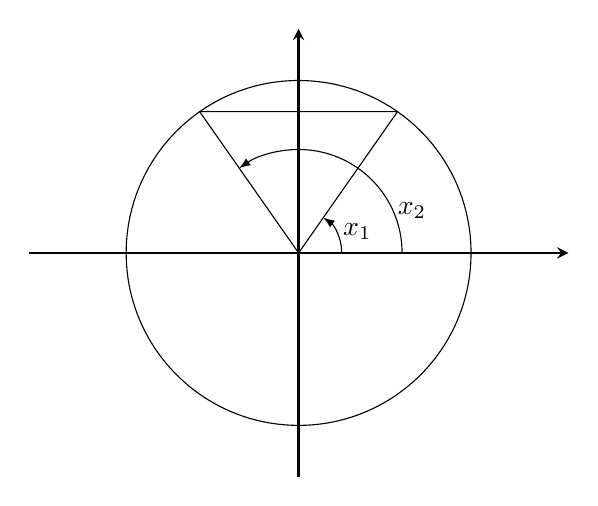
\begin{tikzpicture}
\begin{axis}[
standard,
xmin=-1, xmax=1,
ymin=-1, ymax=1,
xtick={\empty}, ytick={\empty},
axis equal]
\draw[] (0,0) circle [radius=1];
\draw[] (0,0) -- (55:1) -- (125:1) -- cycle;
\coordinate (P) at (55:1 -| 0,0);
\draw[very thick] (0,0) -- (P);
\draw[-latex] (0.25,0) arc [start angle=0, end angle=55, radius=0.25] node[pos=0.25, above right=-22pt]{$x_1$};
\draw[-latex] (0.6,0) arc [start angle=0, end angle=125, radius=0.6] node[pos=0.15,above right=-28pt]{$x_2$};
\end{axis}
\end{tikzpicture}
\end{center}

In order to define $\sin^{-1}$, we restrict the domain of the sine function so that

\begin{enumerate}
\item[(1)] We'll cover all values in the range of $\sin x:[-1,1]$.
\item[(2)] The truncated function will be monotonic on the selected domain, and therefore $1\to1$.
\end{enumerate}

We know from the sinusoidal behavior - and boundedness - of the derivative of sine (literally cosine) that sine has an uncountable number of regions which satisfy these properties - which one do we choose? Well, as we looked at last class, sine is an odd function... For reasons of it being convienient to work with odd functions in certain circumstances, mathematicians have decided to choose the region $[-\pi/2,\pi/2]$ for defining the arcsine function - as it retains the symmetrical properties of sine. Our Math Professor said that another perk of this region is that both graphs intersect the origin in it too, though I would argue that this follows from sine being a continuous odd function.

\vspace{10pt}

We also looked at how sine has a slope of one at the origin. This is proved geometrically in Stewart when we use the Squeeze Theorem to demonstrate that $\lim_{x\to0}\sin x/x=1$. Essentially, $x<\sin x$ for all $-\pi/2<x<0$, and $x>\sin x$ for all $0<x<\pi/2$. We could graph the functions $f(x)=x$ and $g(x)=\sin x$ and see this. The unit circle geometry of this claim is shown below as well - remember that the absolute value of $x$ is greater than the absolute value of $\sin x$ in our truncated interval, $[\pi/2,\pi/2]$, and that this is because the surface area of an inscribed shape is always less than the one containing it, provided that they do not bend in on themselves. That was a bit of a hand wavy explanation on my part about the surface area of inscribed shapes, so I will try and find some more rigorous resources on it for the next note.

\begin{center}
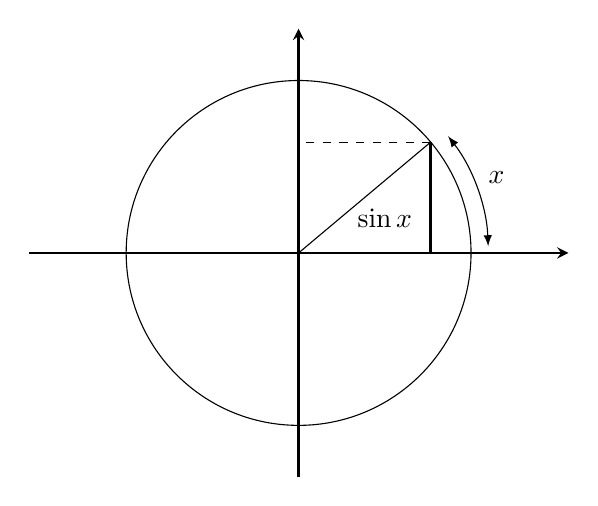
\begin{tikzpicture}
\begin{axis}[
standard,
xmin=-1, xmax=1,
ymin=-1, ymax=1,
xtick={\empty}, ytick={\empty},
axis equal]
\draw[] (0,0) circle [radius=1];
\draw[] (0,0) -- (40:1);
\coordinate (Y) at (40:1 -| 0,0);
\draw[dashed] (40:1) -- (Y);
\coordinate (X) at (40:1 |- 0,0);
\draw[very thick] (40:1) -- (X);
\draw[latex-latex] (2:1.1) arc [start angle=2, end angle=38, radius=1.1] node[pos=0.45,above right=-20pt]{$x$};
\node at (0.5,0.2) {$\sin x$};
\end{axis}
\end{tikzpicture}
\end{center}

And so we define arcsine to be on the domain $[-1,1]$, since it exhibits useful properties on that interval.

\begin{center}
\begin{tikzpicture}
\begin{axis}[
standard,
xmin=-1.57, xmax=4.71,
ymin=-1, ymax=1,
xtick={\empty}, ytick={\empty}]
\addplot[domain=-pi/2:pi/2,samples=200] {sin(deg(x))};
\addplot[domain=pi/2:5,samples=200,dashed] {sin(deg(x))};
\addplot[domain=-3:-pi/2,samples=200,dashed] {sin(deg(x))};
\draw[dashed] (-pi/2,0) -- (-pi/2,-1) node[pos=0,above]{$-\pi/2$};
\draw[dashed] (pi/2,0) -- (pi/2,1) node[pos=0,below]{$\pi/2$};
\end{axis}
\end{tikzpicture}
\end{center}

And to obtain the graph of arcsine, we just flip that truncated region of sine about the line $y=x$:

\begin{center}
\begin{tikzpicture}
\begin{axis}[
standard,
xmin=-1, xmax=1,
ymin=-1.6, ymax=1.6,
xtick={\empty}, ytick={\empty}]
\addplot[domain=-1:1,samples=200] {asin(x)/180*pi};
\draw[dashed] (1,pi/2) -- (1,pi/2 -| 0,0) node[pos=1,left]{$\pi/2$};
\draw[dashed] (1,pi/2) -- (1,pi/2 |- 0,0) node[pos=1,below]{$1$};
\end{axis}
\end{tikzpicture}
\end{center}

$f^{-1}(x)\equiv\arcsin(x)\equiv\sin^{-1}x$ is a function, such that: $\arcsin x=y$ means $\sin y=x$.

\vspace{10pt}

After going over the theoretical aspects of inverse trigonometric functions, it can be easy to be intimidated - I know I was when first exposed to it. So let me just emphasize that all an inverse trigonometric function is is just a function that "undoes" the parent trigonometric function function - the input and output sets are essentially reversed.

\vspace{10pt}

Now, lets apply our general knowledge of inverse trig. functions to some special cases:


\vspace{10pt}

{\bf{}EXAMPLE} Evaluate $y=\arcsin\frac{1}{2}$

\vspace{10pt}

$y$ is such an angle (arc) that $\sin y=\frac{1}{2}$ and $-\pi/2<y<\pi/2$.

\begin{center}
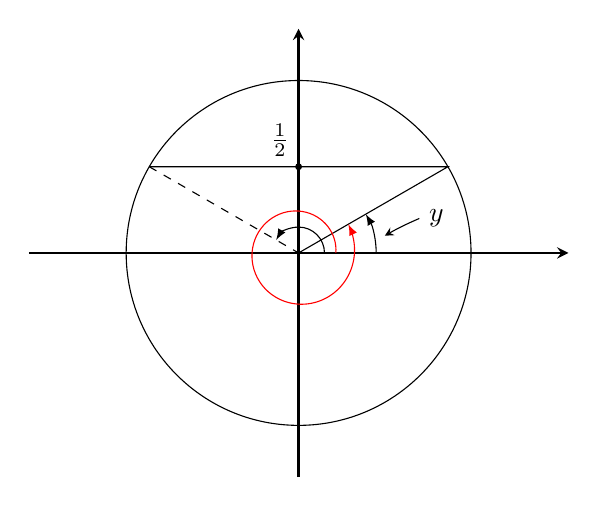
\begin{tikzpicture}
\begin{axis}[
standard,
xmin=-1, xmax=1,
ymin=-1, ymax=1,
xtick={\empty}, ytick={\empty},
axis equal]
\draw[] (0,0) circle [radius=1];
\draw[] (180-30:1) -- (30:1) -- (0,0);
\draw[dashed] (180-30:1) -- (0,0);
\node[above left] at (0,0.5) {$\frac{1}{2}$};
\fill[] (0,0.5) circle [radius=0.02];
\draw[-latex,domain=360+360:750+360,variable=\t,smooth,samples=75,red] plot ({\t}: {0.0003*\t});
\draw[-latex] (0.15,0) arc [start angle=0, end angle=180-30,radius=0.15];
\draw[-latex] (0.45,0) arc [start angle=0, end angle=30,radius=0.45];
\draw[stealth-] (0.5,0.1)  to[bend left=3pt] (0.7,0.2);
\node[right] at (0.7,0.2) {$y$};
\end{axis}
\end{tikzpicture}
\end{center}

From our discussion of special triangles last class, we are equipped to solve this. As was gone over, 0.5 is a special trigonometric ratio that corresponds to the 30-60 degree triangle. And for sine, the angle is pi over six. $\therefore y=\frac{\pi}{6}$. It is important to remember that the angle \textit{must} be in the range of the inverse, even though there are angles whose sines also have this value - we defined the inverse with these limitations intentionally and should keep to it unless there is a practical reason not to.

\vspace{10pt}

After this example, Our Math Professor emphasized the point that on the unit circle, an arclength is of the exact same magnitude as the angle it subtends - due to the radius being one. If you have an angle of three and a half radians, the corresponding arc would be three and a half units in length.

\vspace{10pt}

{\bf{}EXAMPLE} Evaluate $\sin(\arcsin\frac{1}{3})=\frac{1}{3}$

\vspace{10pt}

One third is within the range of the sine function, therefore the inverse sine function can be applied to it. Since sine "undoes" its inverse, we are left with one third.

\vspace{10pt}

{\bf{}EXAMPLE} Evaluate $\arcsin(\sin\frac{2\pi}{3})\color{red}\neq\color{black}\frac{2\pi}{3}$

\vspace{10pt}

In English, $\arcsin(\sin\frac{2\pi}{3})$ is an angle $\theta:\left\{\begin{array}{c}\sin\theta=\sin\frac{2\pi}{3}\\-\pi/2\leq\theta\leq\pi/2\end{array}\right.$ (Our Math Professor introduced the colon (``:") notation which is another way of saying  ``such that").

\begin{center}
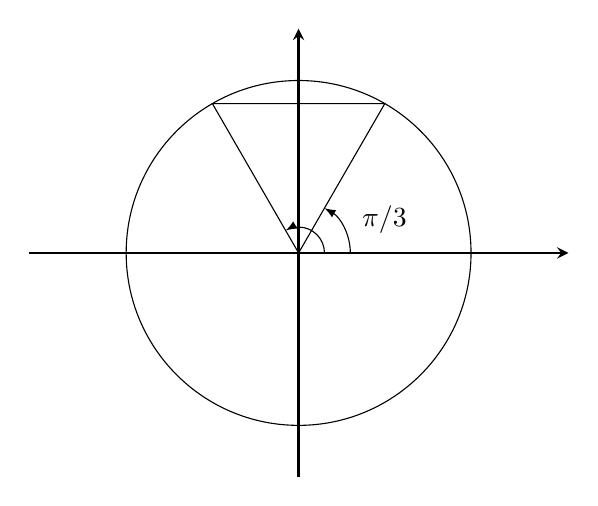
\begin{tikzpicture}
\begin{axis}[
standard,
xmin=-1, xmax=1,
ymin=-1, ymax=1,
xtick={\empty}, ytick={\empty},
axis equal]
\draw[] (0,0) circle [radius=1];
\draw[] (0,0) -- (60:1) -- (180-60:1) -- cycle;
\draw[very thick] (0,0) -- (60:1 -| 0,0);
\draw[-latex] (0.15,0) arc [start angle=0, end angle=120, radius=0.15];
\draw[-latex] (0.3,0) arc [start angle=0, end angle=60, radius=0.3] node[pos=0.15,right=-8pt]{$\pi/3$};
\end{axis}
\end{tikzpicture}
\end{center}

\[\Rightarrow\frac{2\pi}{3}=\pi-\pi/3\therefore\theta=\pi/3\]

In my humble opinion, the more intuitive approach - in comparison to the logic above - would be to find the smallest angle with that sine. This would ensure us getting a result which corresponds to the truncated region of sine.

\vspace{10pt}

{\bf{}EXAMPLE} Evaluate $\arcsin(\sin4)$

\begin{center}
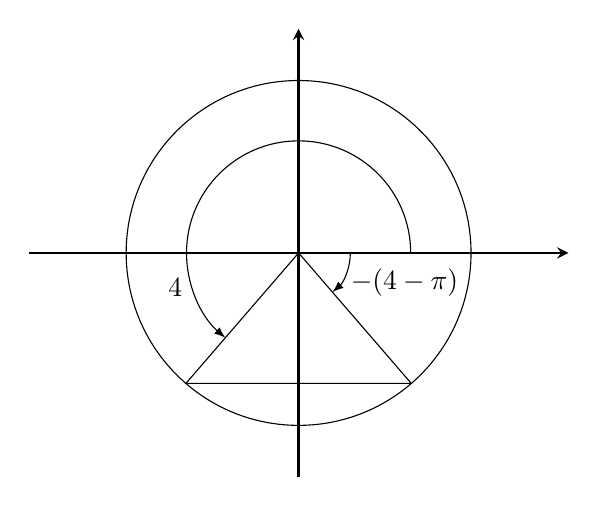
\begin{tikzpicture}
\begin{axis}[
standard,
xmin=-1, xmax=1,
ymin=-1, ymax=1,
xtick={\empty}, ytick={\empty},
axis equal]
\draw[] (0,0) circle [radius=1];
\draw[] (0,0) -- (2*360/pi:1) -- (-2*360/pi+180:1) -- cycle;
\draw[very thick] (0,0) -- (2*360/pi:1 -| 0,0);
\draw[-latex] (0.65,0) arc [start angle=0, end angle=2*360/pi, radius=0.65];
\node[left] at (180+18:0.65) {$4$};
\draw[-latex] (0.3,0) arc [start angle=0, end angle=-2*360/pi+180, radius=0.3];
\node[right] at (-35:0.3) {$-(4-\pi)$};
\end{axis}
\end{tikzpicture}
\end{center}

So, $\arcsin(\sin4)=y:\ \sin y=\sin 4\textnormal{ and }-\pi/2\leq y\leq\pi/2$ (recall that ``:" means ``such that")

\vspace{10pt}

So, as we did with sine, we also need to define an inverse function for the cosine function - which is like sine in that it is bounded, continuous, and sinusoidal. If you draw the cosine function (see the diagram below, which I replicated from our textbook), then you may notice that if we apply the same domain restraints as we did with sine, that we would not have a $1\to1$ function. Unfortunately, there is no way to preserve the symmetry of cosine when defining its inverse. Instead, we define it basically the same way, but shifted so the region is $1\to1$.

\begin{center}
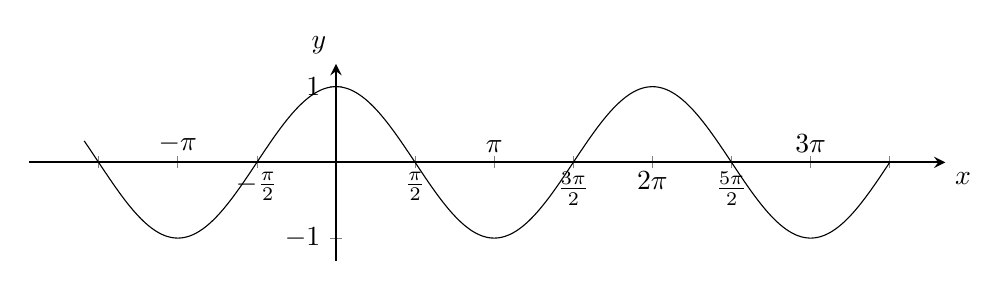
\begin{tikzpicture}
\begin{axis}[
standard,
xmin=-4, xmax=10,
xtick={-3.14159*3/2,-3.14159,-3.14159/2,3.14159/2,3.14159,3.14159*3/2,3.14159*2,3.14159*5/2,3.14159*3,3.14159*7/2}, ytick={-1,1},
xticklabels={}, yticklabels={$-1$,$1$},
xlabel={$x$}, ylabel={$y$},
  width=.96\linewidth,
    height=2.5cm,
    scale only axis=true]
\addplot[domain=-5:11,samples=300] {cos(deg(x))};
\node[above] at (-3.14159,0) {$-\pi$};
\node[above] at (3.14159,0) {$\pi$};
\node[above] at (3.14159*3,0) {$3\pi$};
\node[below] at (-3.14159/2,0) {$-\frac{\pi}{2}$};
\node[below] at (3.14159/2,0) {$\frac{\pi}{2}$};
\node[below] at (3.14159*3/2,0) {$\frac{3\pi}{2}$};
\node[below] at (3.14159*2,0) {$2\pi$};
\node[below] at (3.14159*5/2,0) {$\frac{5\pi}{2}$};
\end{axis}
\end{tikzpicture}
\end{center}

We could have looked at the unit circle geometry, but the Cartesian graph is very illuminating for this. For reasons of keeping the domain positive, and working with smaller (simpler) numbers, math people choose the region $[0,\pi]$. Since cosine is monotonic on this interval, we can define an inverse.

\[f^{-1}(x)\equiv\arccos x\equiv\cos^{-1}x\]

Such that $y=\arccos x$ means $y$ is such an angle that $\cos y=x$ and $0\leq y\leq\pi$.

\vspace{10pt}

{\bf{}EXAMPLE} Evaluate $y=\arccos(\cos\frac{4\pi}{3})$

\vspace{10pt}

$y$ is such an angle that $\cos y=\cos(4\pi/3)$ and $0\leq y\leq\pi$.

\begin{center}
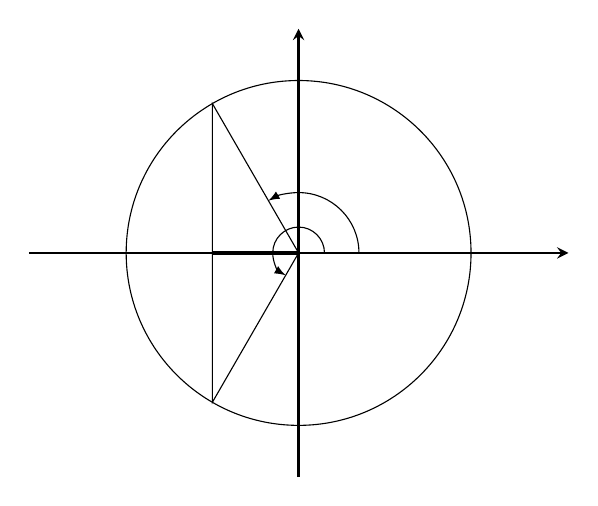
\begin{tikzpicture}
\begin{axis}[
standard,
xmin=-1, xmax=1,
ymin=-1, ymax=1,
xtick={\empty}, ytick={\empty},
axis equal]
\draw[] (0,0) circle [radius=1];
\draw[] (0,0) -- (120:1) -- (240:1) -- cycle;
\draw[very thick] (0,0) -- (120:1 |- 0,0);
\draw[-latex] (0.15,0) arc [start angle=0, end angle=240, radius=0.15];
\draw[-latex] (0.35,0) arc [start angle=0, end angle=120, radius=0.35];
\end{axis}
\end{tikzpicture}
\end{center}

\[\therefore y=2\pi/3\]

{\bf{}EXAMPLE} For homework, evaluate $y=\arccos(\cos4.5)$





\end{document}